\newpage

\anonchapter{Лабораторная работа №2}
\setcounter{chapter}{2}

\begin{center}
Определение ширины запрещённой зоны полупроводника \\
(4 часа)
\end{center}

\section{Цель работы}
Определение ширины запрещённой зоны в кремний-углеродных плёнках на основе измерения температурной зависимости электропроводности.

\section{Теоретическая часть}
\subsection{Температурная зависимость электропроводности}

Характерным признаком, отличающим полупроводник от металла, является увеличение электропроводности полупроводников при повышении температуры.

Для полупроводника с одним выделенным типом проводимости удельную электропроводность можно представить в виде:
\begin{equation}
\sigma = e n \mu
\end{equation}
где $e$ - заряд электрона, $n$ - концентрация примеси, $\mu$ - подвижность носителей заряда.

При рассмотрении электропроводности в образце с обоими типами носителей, необходимо учитывать вклады каждого из них:
\begin{equation}
\sigma = e n \mu_{n} + e p \mu_{p}
\end{equation}

Для анализа температурной зависимости полупроводника рассмотрим влияние температуры на подвижность и концентрацию свободных носителей заряда (СНЗ).

\subsection{Температурная зависимость конценрации СНЗ}

Для примера рассмотрим примесный полупроводник n-типа. На рисунке \ref{pic2_zone} показана энергетическая диаграмма донорного полупроводника. Общий вид зависимости концентрации от температуры для невырожденного полупроводника с одним типом донорной примеси представлен на рисунке \ref{pic2_n_T}.

\begin{figure}[h!]\centering
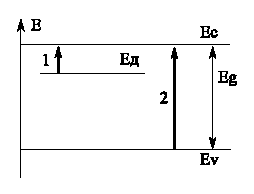
\includegraphics[height=4cm]{pic2_zone.eps}
\caption{Зонная диаграмма с одним типом донорной примеси}
\label{pic2_zone}
\end{figure}

\begin{figure}[h!]\centering
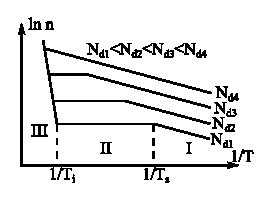
\includegraphics[height=4cm]{pic2_n_T.eps}
\caption{Общий вид температурной зависимости концентрации для невырожденного полупроводника с одним типом примеси}
\label{pic2_n_T}
\end{figure}

Из зависимости $\ln n = f(\frac{1}{T})$ можно выделить три характерных температурных интервала.

\paragraph{I. Область примесной ионизации.}
При абсолютном нуле валентная зона полупроводника целиком заполнена электронами. В зоне проводимости нет свободных носителей. При повышении температуры электроны переходят с уровней донорной примеси в зону проводимости, концентрация свободных электронов повышается. Это процесс называется ионизацией атомов примеси и продолжается вплоть до температуры истощения примеси $T = T_{s}$. В этой области
\begin{equation}
n = \sqrt{\frac{N_{c}N_{d}}{2}} \exp{\left( -\frac{\Delta E_{d}}{2 k T} \right)}
\end{equation}
где $N_{c} = 2 \left( \frac{2 \pi m_{dn}^{*} k T}{h^2} \right) ^ \frac{3}{2}$ - эффективная плотность состояний в зоне проводимости, $\Delta E_{d}$ - энергия ионизации донорной примеси, $N_{d}$ - концентрация примеси.

\paragraph{II. Область истощения примеси.}
В области температур $T_{s} < T < T_{i}$ донорная примесь полностью ионизована, но собственная ионизация ещё не началась. Поэтому концентрация свободных электронов постоянна и равна $N_{d}$.
Ширина области истощения зависит от концентрации ионизирующей примеси и её энергии ионизации. При увеличении этих величин температурный интервал области истощения будет уменьшаться. При достаточно больших значениях $N_{d}$ он может исчезнуть полностью.

\paragraph{III. Область собственной ионизации.}
В области высоких температур $(T > T_{i})$, когда энергия теплового движения электронов становится сопоставимой с шириной запрещённой зоны $(k T \approx E_{g})$, электроны начинают переходить из валентной зоны в зону проводимости, из-за чего концентрация свободных носителей резко возрастает. Происходит ионизация атомов основного вещеста.

\begin{equation}
n_{i} = \sqrt{N_{c} N_{v}} \exp{\left( -\frac{E_{g}}{k T} \right)} \sim T^{\frac{3}{2}} \exp{\left( -\frac{E_{g}}{k T} \right)}
\label{eq2_ni_T}
\end{equation}

Ширина запрещённой зоны также зависит от температуры. Для большинства полупроводников величина $E_{g}$ сложным образом снижается с температурой, однако в широком диапазоне температур она может быть аппроксимирована прямой линией:
\begin{equation}
E_{g}(T) = E_{g}(0) + \alpha T
\label{eq2_E_T}
\end{equation}
где $E_{g}(0)$ - значение, которое можно получить экстраполяцией температурной зависимости ширины запрещённой зоны на значение 0\textdegree К, $\alpha$ - температурный коэффициент изменения ширины запрещённой зоны, обычно отрицателен и составляет десятые доли мэВ/К.

На рисунке \ref{pic2_E_T} показана температурная зависимость ширины запрещённой зоны в кремнии.

\begin{figure}[h!]\centering
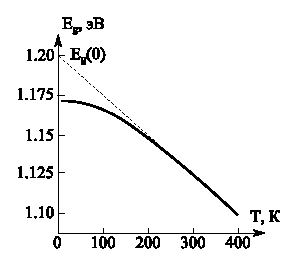
\includegraphics[height=4cm]{pic2_E_T.eps}
\caption{Температурная зависимость ширины запрещённой зоны для кремния}
\label{pic2_E_T}
\end{figure}

Подставляя (\ref{eq2_E_T}) в (\ref{eq2_ni_T}) получаем:
\begin{equation}
n_{i} = \sqrt{N_{c} N_{v}} \exp{\left( -\frac{E_{g}(0) + \alpha T}{k T} \right)} \sim T^{\frac{3}{2}} \exp{\left( -\frac{E_{g}(0)}{k T} \right)} \exp{\left( -\frac{\alpha}{k} \right)}
\end{equation}

\subsection{Температурная зависимость подвижности СНЗ}
Подвижность также зависит от температуры. Характер зависимости определяется доминирующим механизмом рассеяния в полупроводнике при данной температуре. Для большинства механизсов зависимость $\mu(T)$ имеет ярко выраженную степенную зависимость:
\begin{equation}
\mu(T) = \mu_{i} \left( \frac{T}{T_{i}} \right)^{m}
\end{equation}
где $\mu_{i}$ - подвижность при температуре $T = T_{i}$.

Если основным механизмом является рассеяние на ионах примеси, показатель $m = \frac{3}{2}$. Для рассеяния на нейтральных примесях $m = 0$, а для рассеяния на акустических фононах $m = -frac{3}{2}$.